%pdflatex-../thesis.tex
% vim:spell spelllang=en_us

\section{Measurement samples}
\label{appendix:measurement-samples}
\subsection{Measurement \#23}
$100~\Jed{Mb/s}$, $100$ cycles, 6\% failed
\begin{figure}[hp]
	\begin{center}
	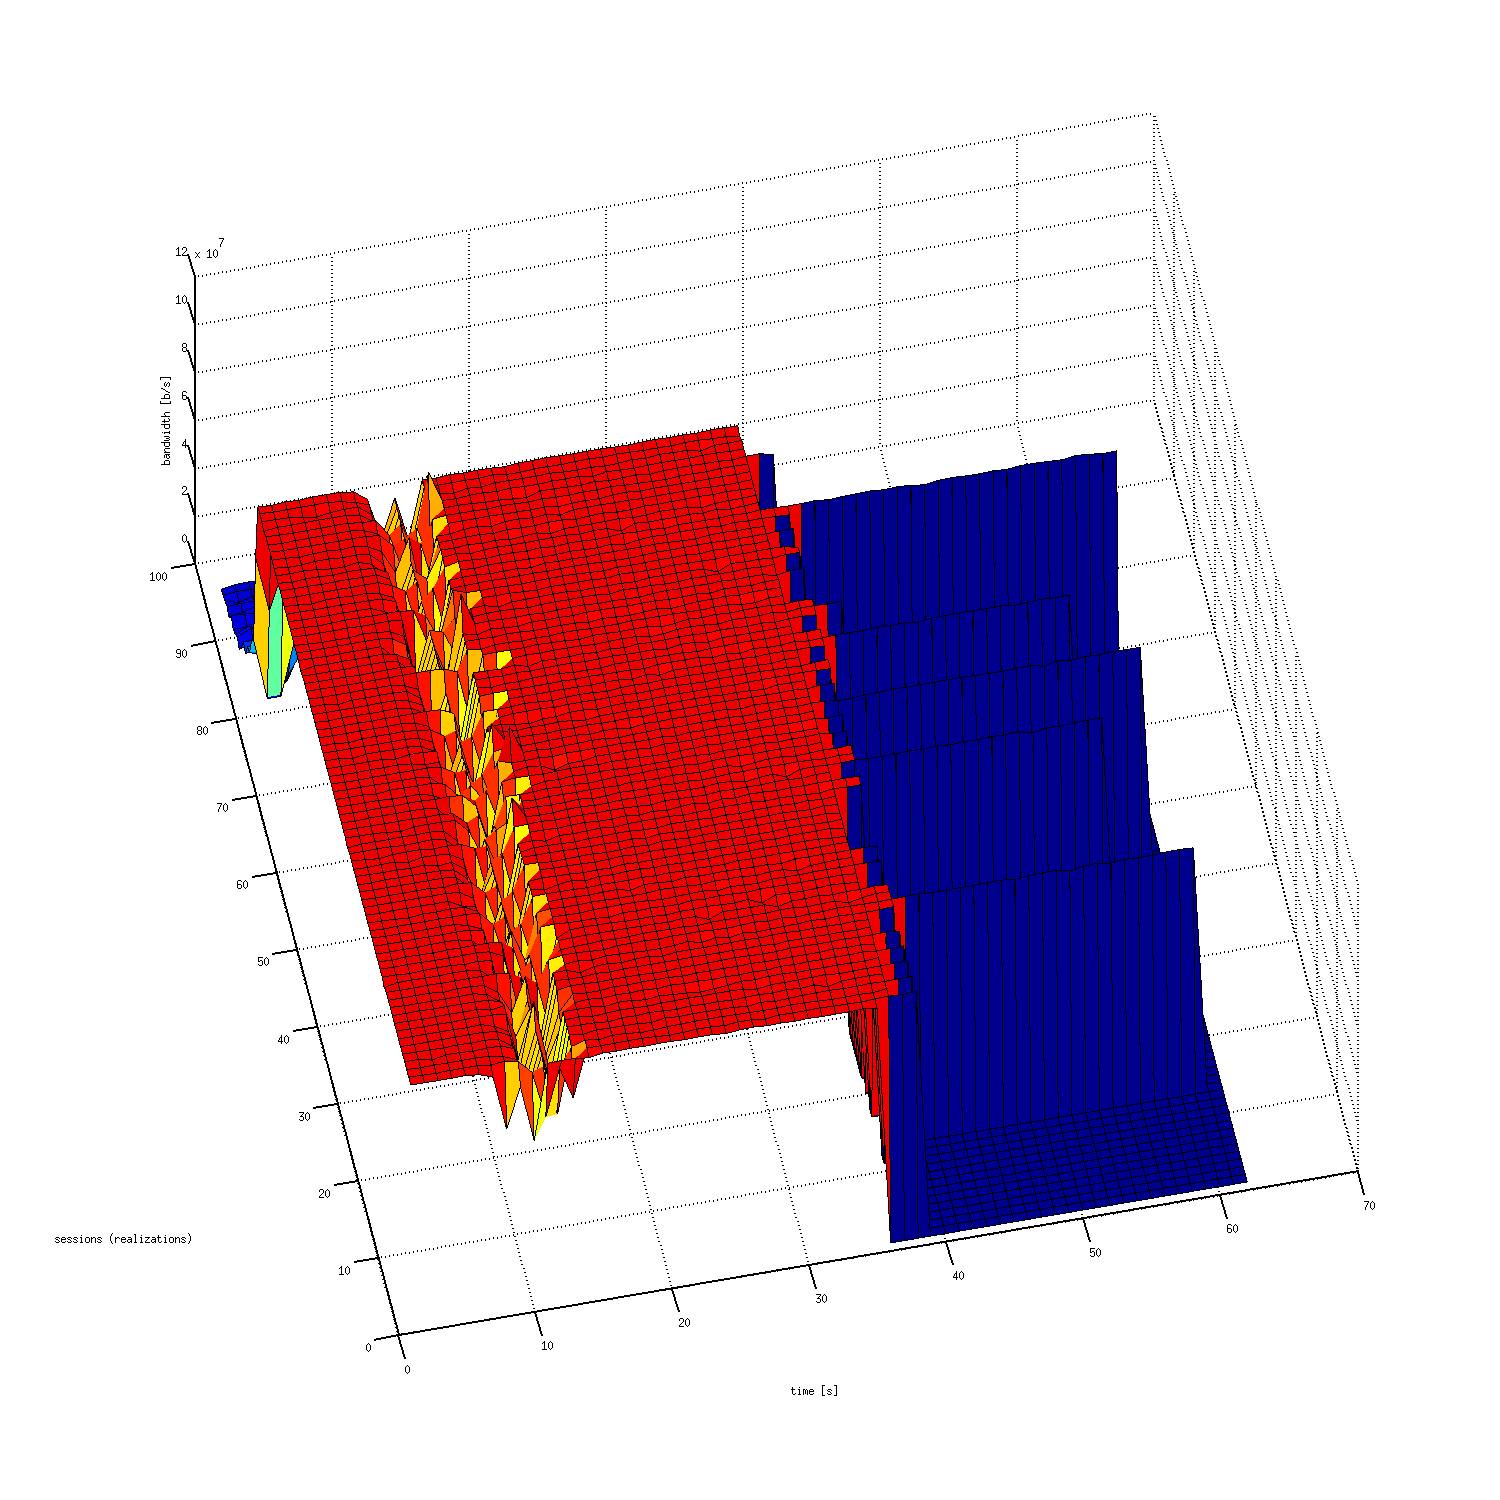
\includegraphics[width=0.9\textwidth]{results-239-3d.png}
	\end{center}
	\caption[]{\#23, bandwidth [b/s]}
	\label{img:results-239-3d.png}
\end{figure}

\begin{figure}[hp]
	\begin{center}
	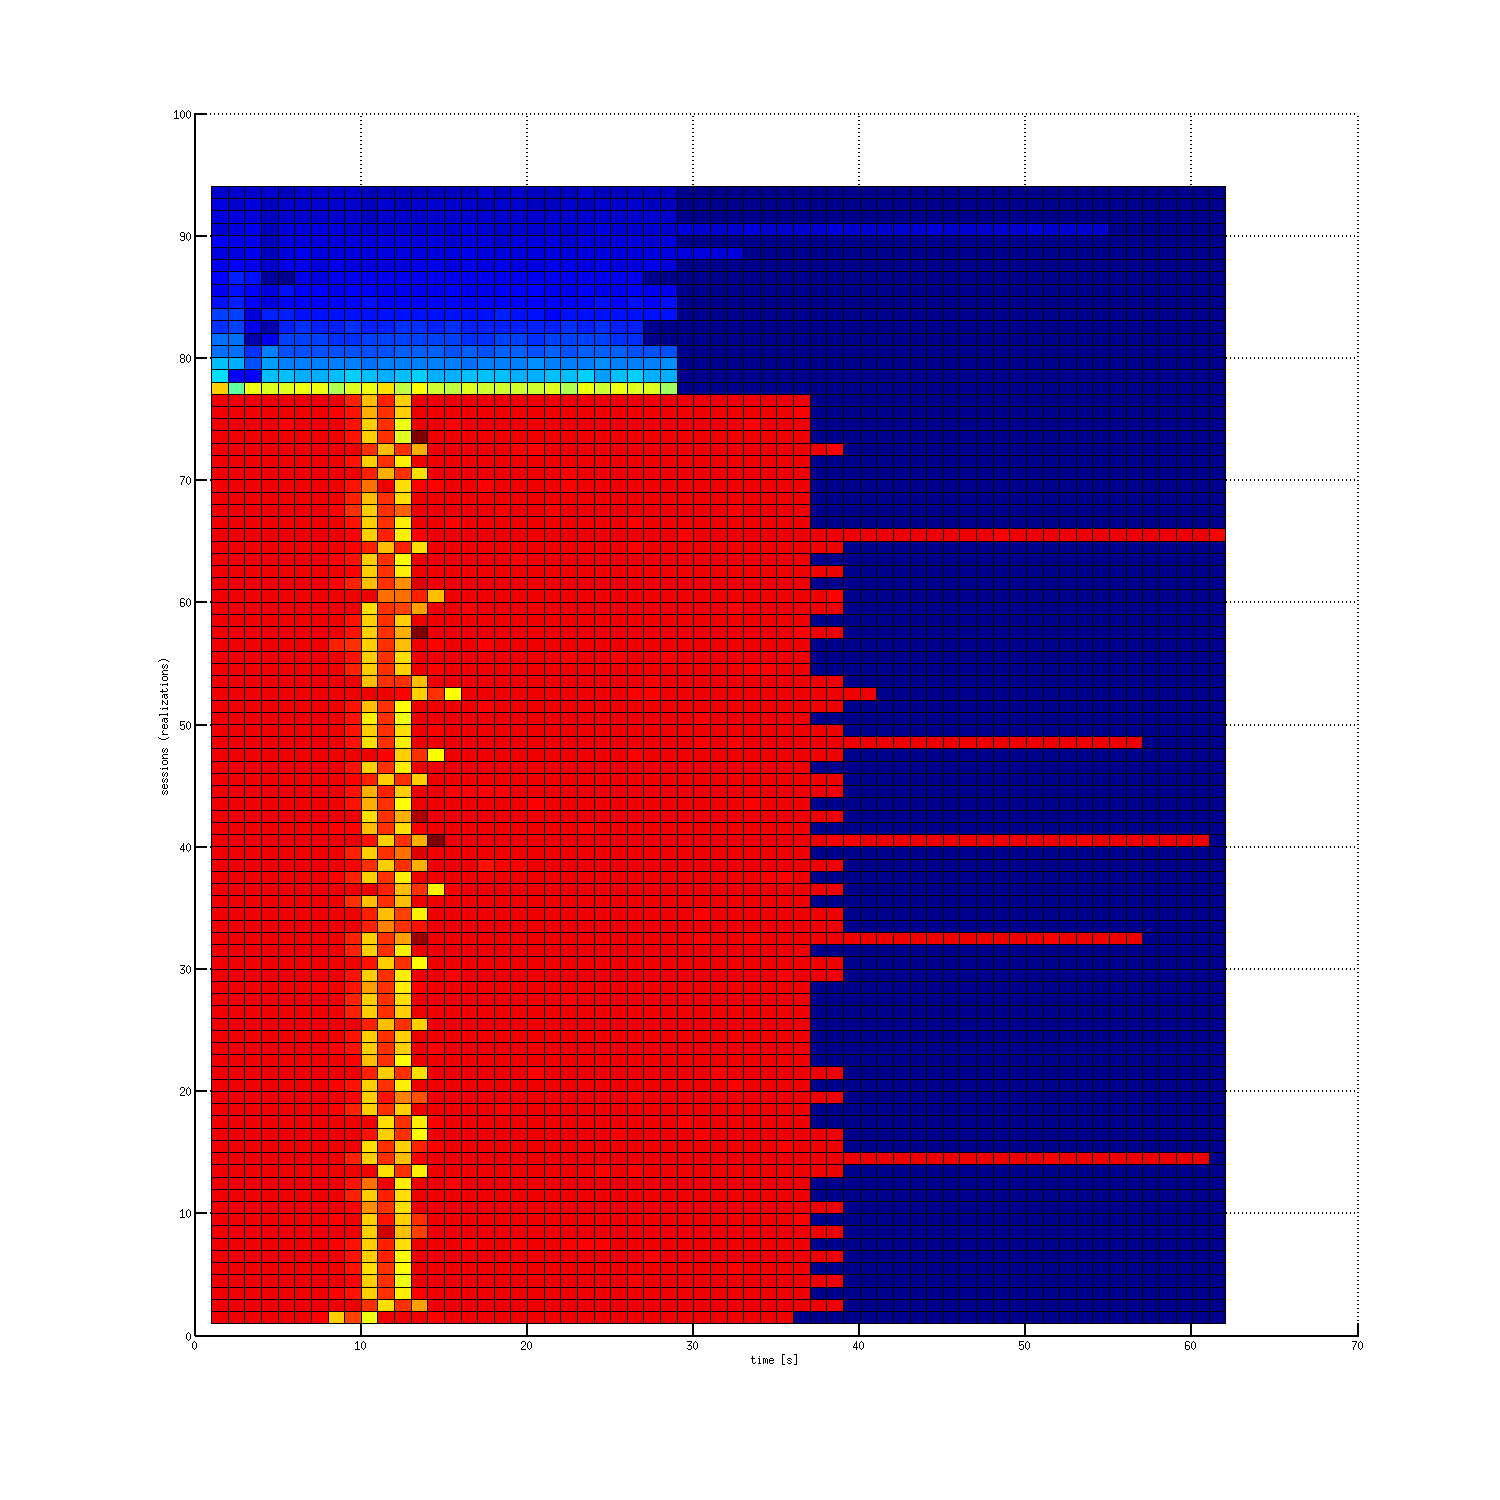
\includegraphics[width=0.9\textwidth]{results-239-2d.png}
	\end{center}
	\caption[]{\#23, bandwidth [b/s] (z axis - color), flat view}
	\label{img:results-239-2d.png}
\end{figure}
\FloatBarrier
\clearpage

% 269
\subsection{Measurement \#26}
$140~\Jed{Mb/s}$, $300$ cycles, 6\% failed
\begin{figure}[hp]
	\begin{center}
	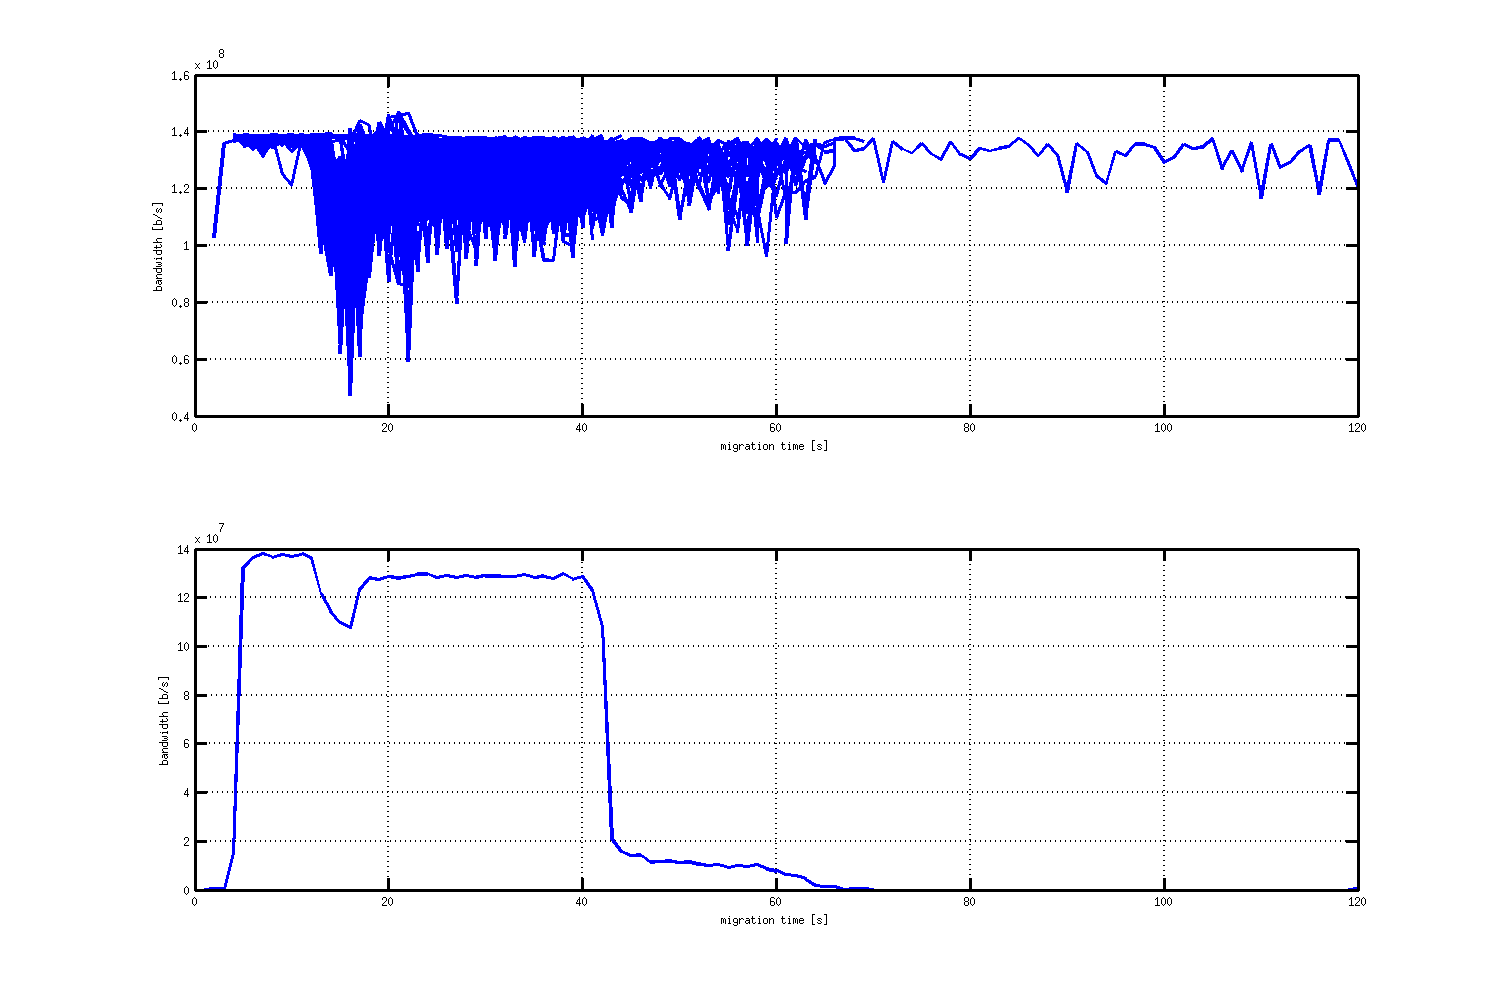
\includegraphics[width=0.9\textwidth]{results-269-all.png}
	\end{center}
	\caption[]{\#26, bandwidth for all sessions (top), average (bottom) [b/s]}
	\label{img:results-269-all.png}
\end{figure}
\begin{figure}[hp]
	\begin{center}
	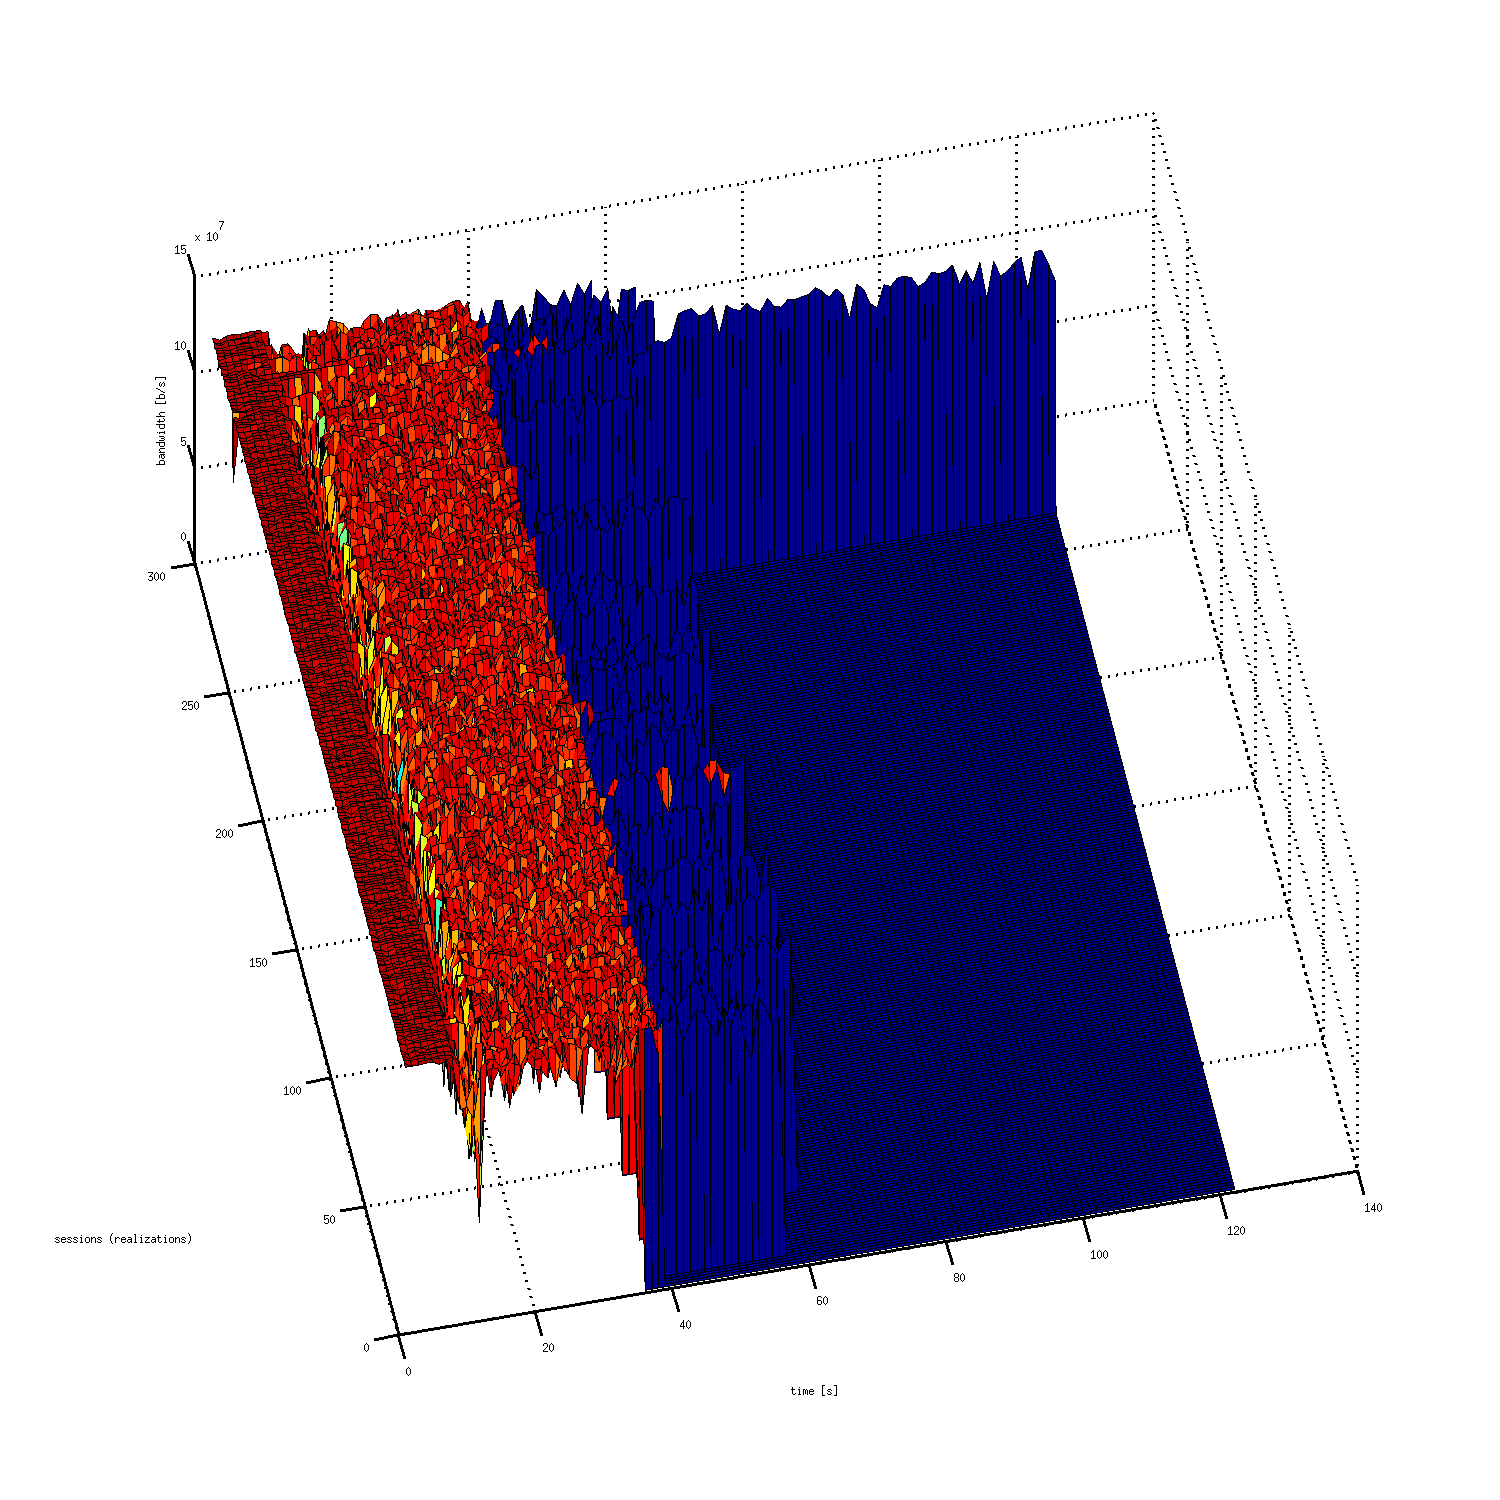
\includegraphics[width=0.9\textwidth]{results-269-3d.png}
	\end{center}
	\caption[]{\#26, bandwidth [b/s]}
	\label{img:results-269-3d.png}
\end{figure}
\begin{figure}[hp]
	\begin{center}
	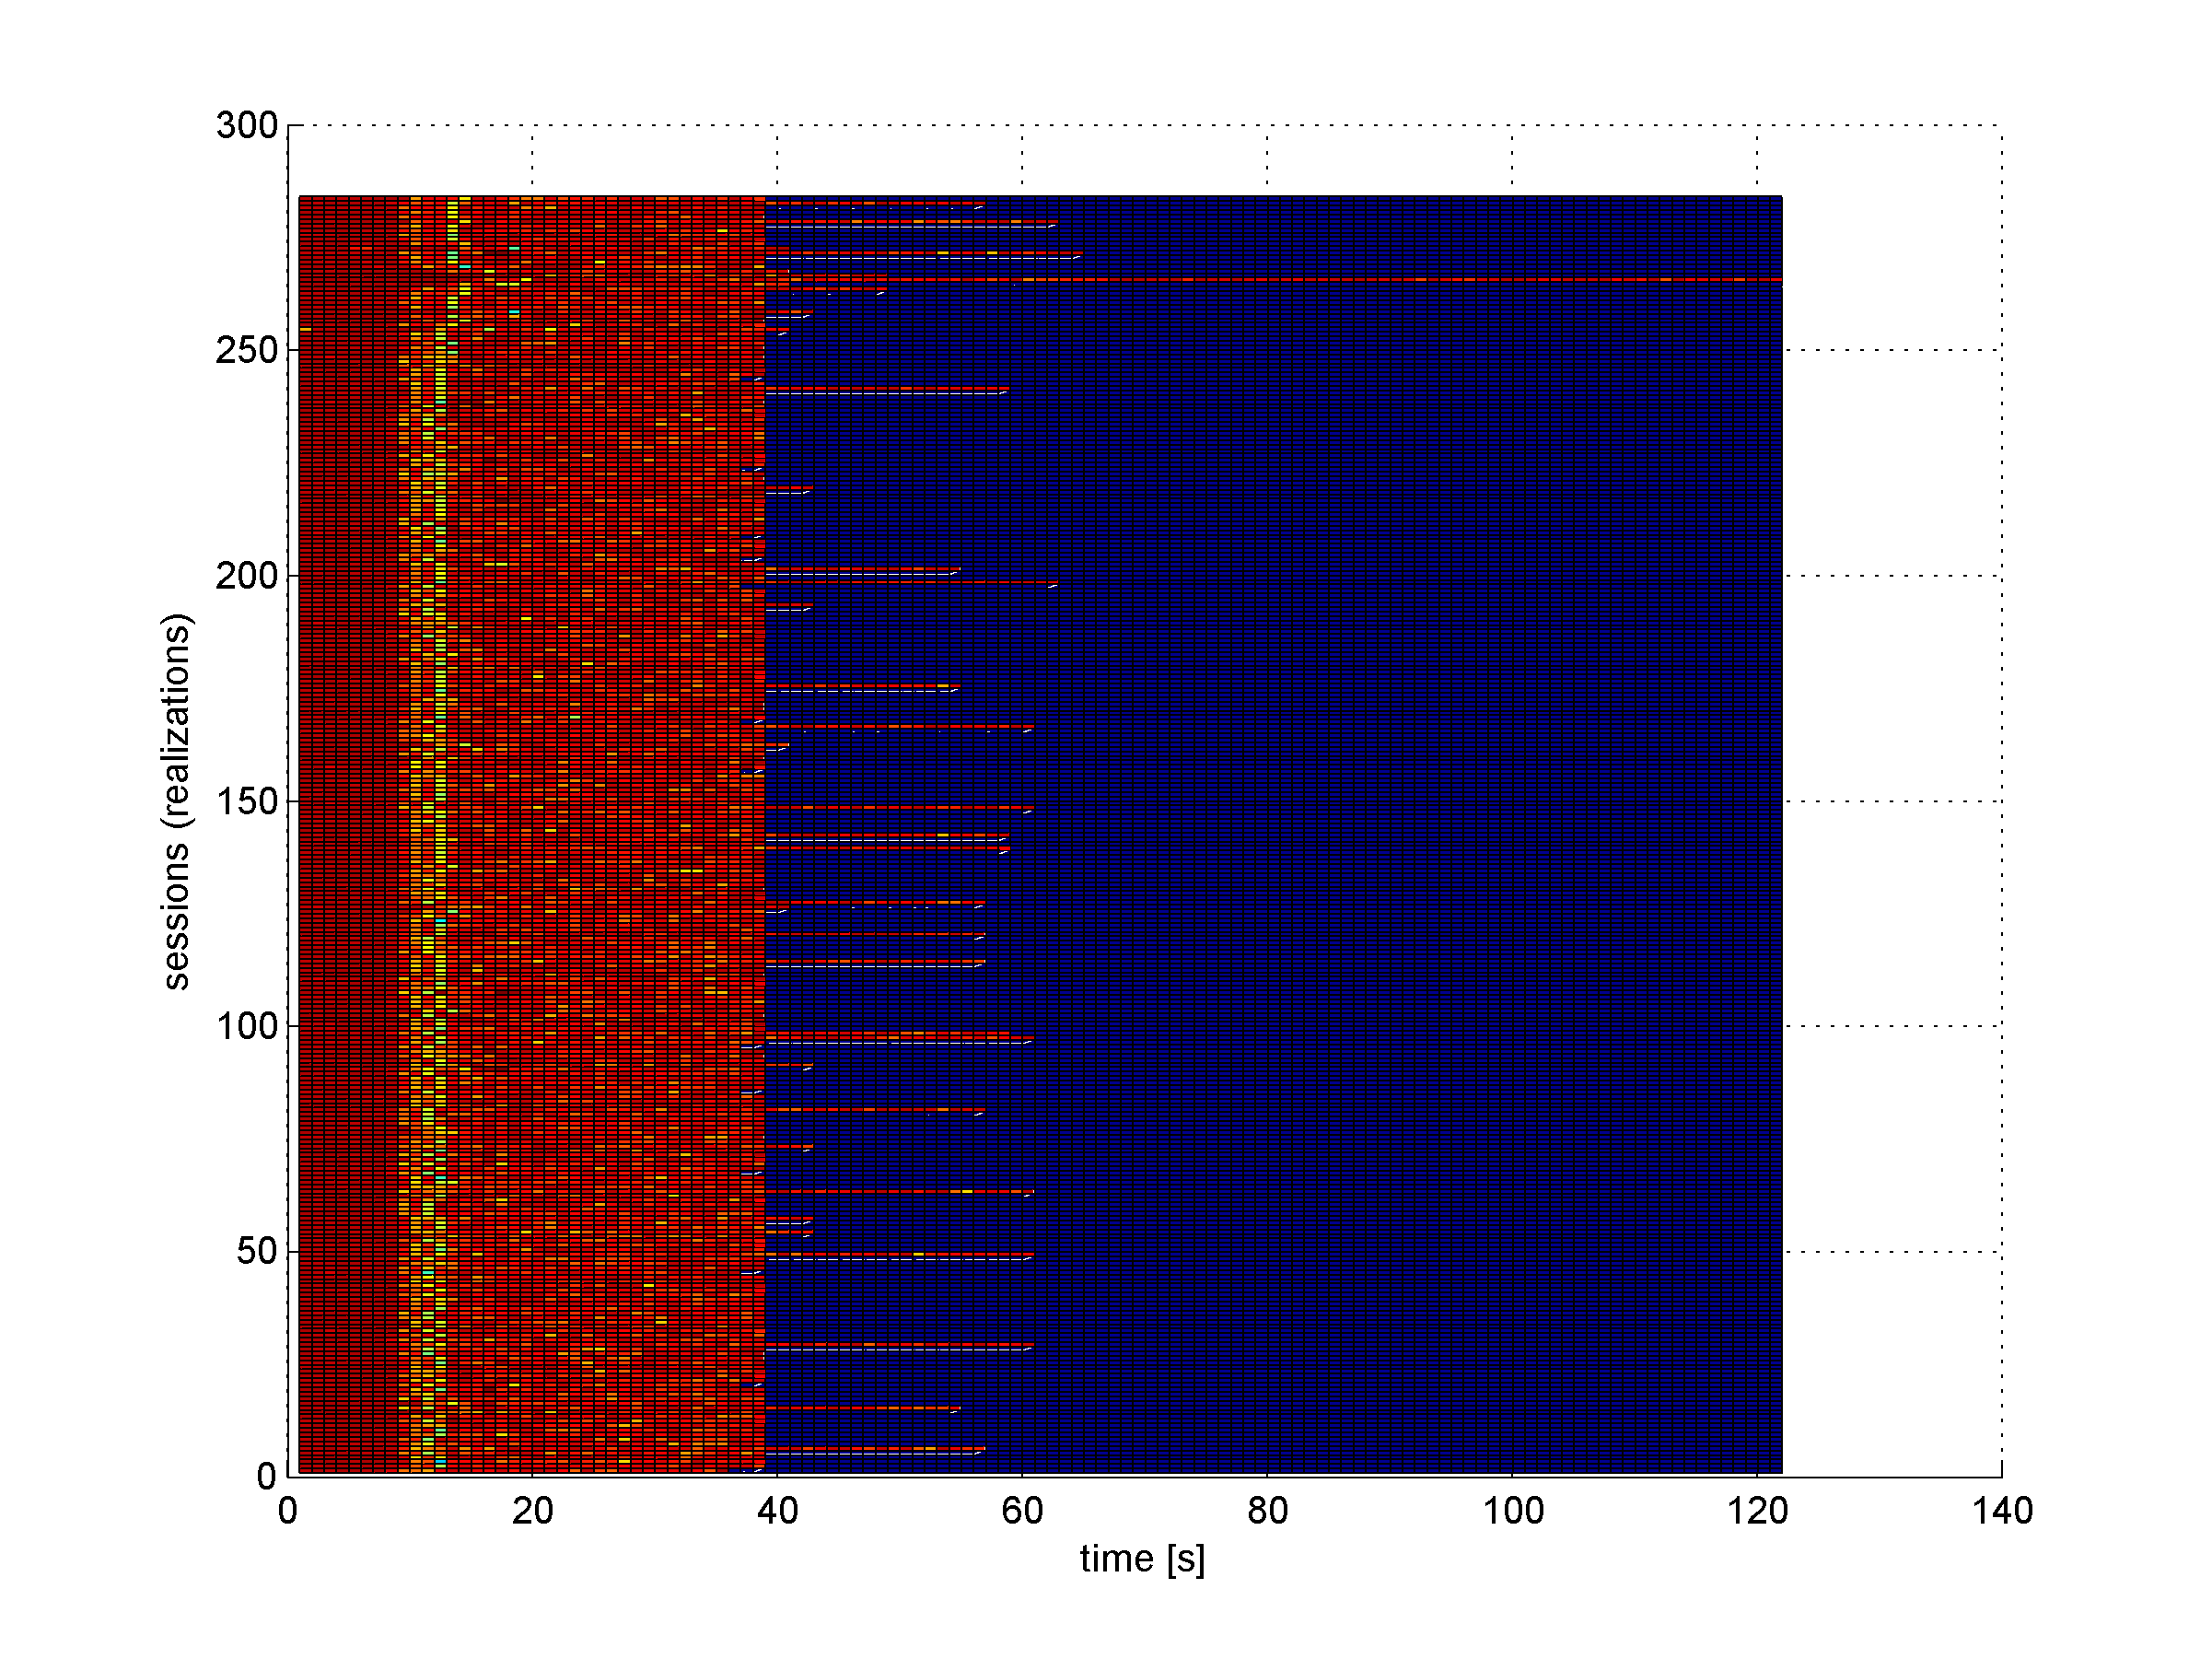
\includegraphics[width=0.9\textwidth]{results-269-2d.png}
	\end{center}
	\caption[]{\#26, bandwidth [b/s] (z axis - color), flat view}
	\label{img:results-269-2d.png}
\end{figure}
\FloatBarrier
\clearpage

% 274
\subsection{Measurement \#27}
$80~\Jed{Mb/s}$, $200$ cycles, 10\% failed
\begin{figure}[hp]
	\begin{center}
	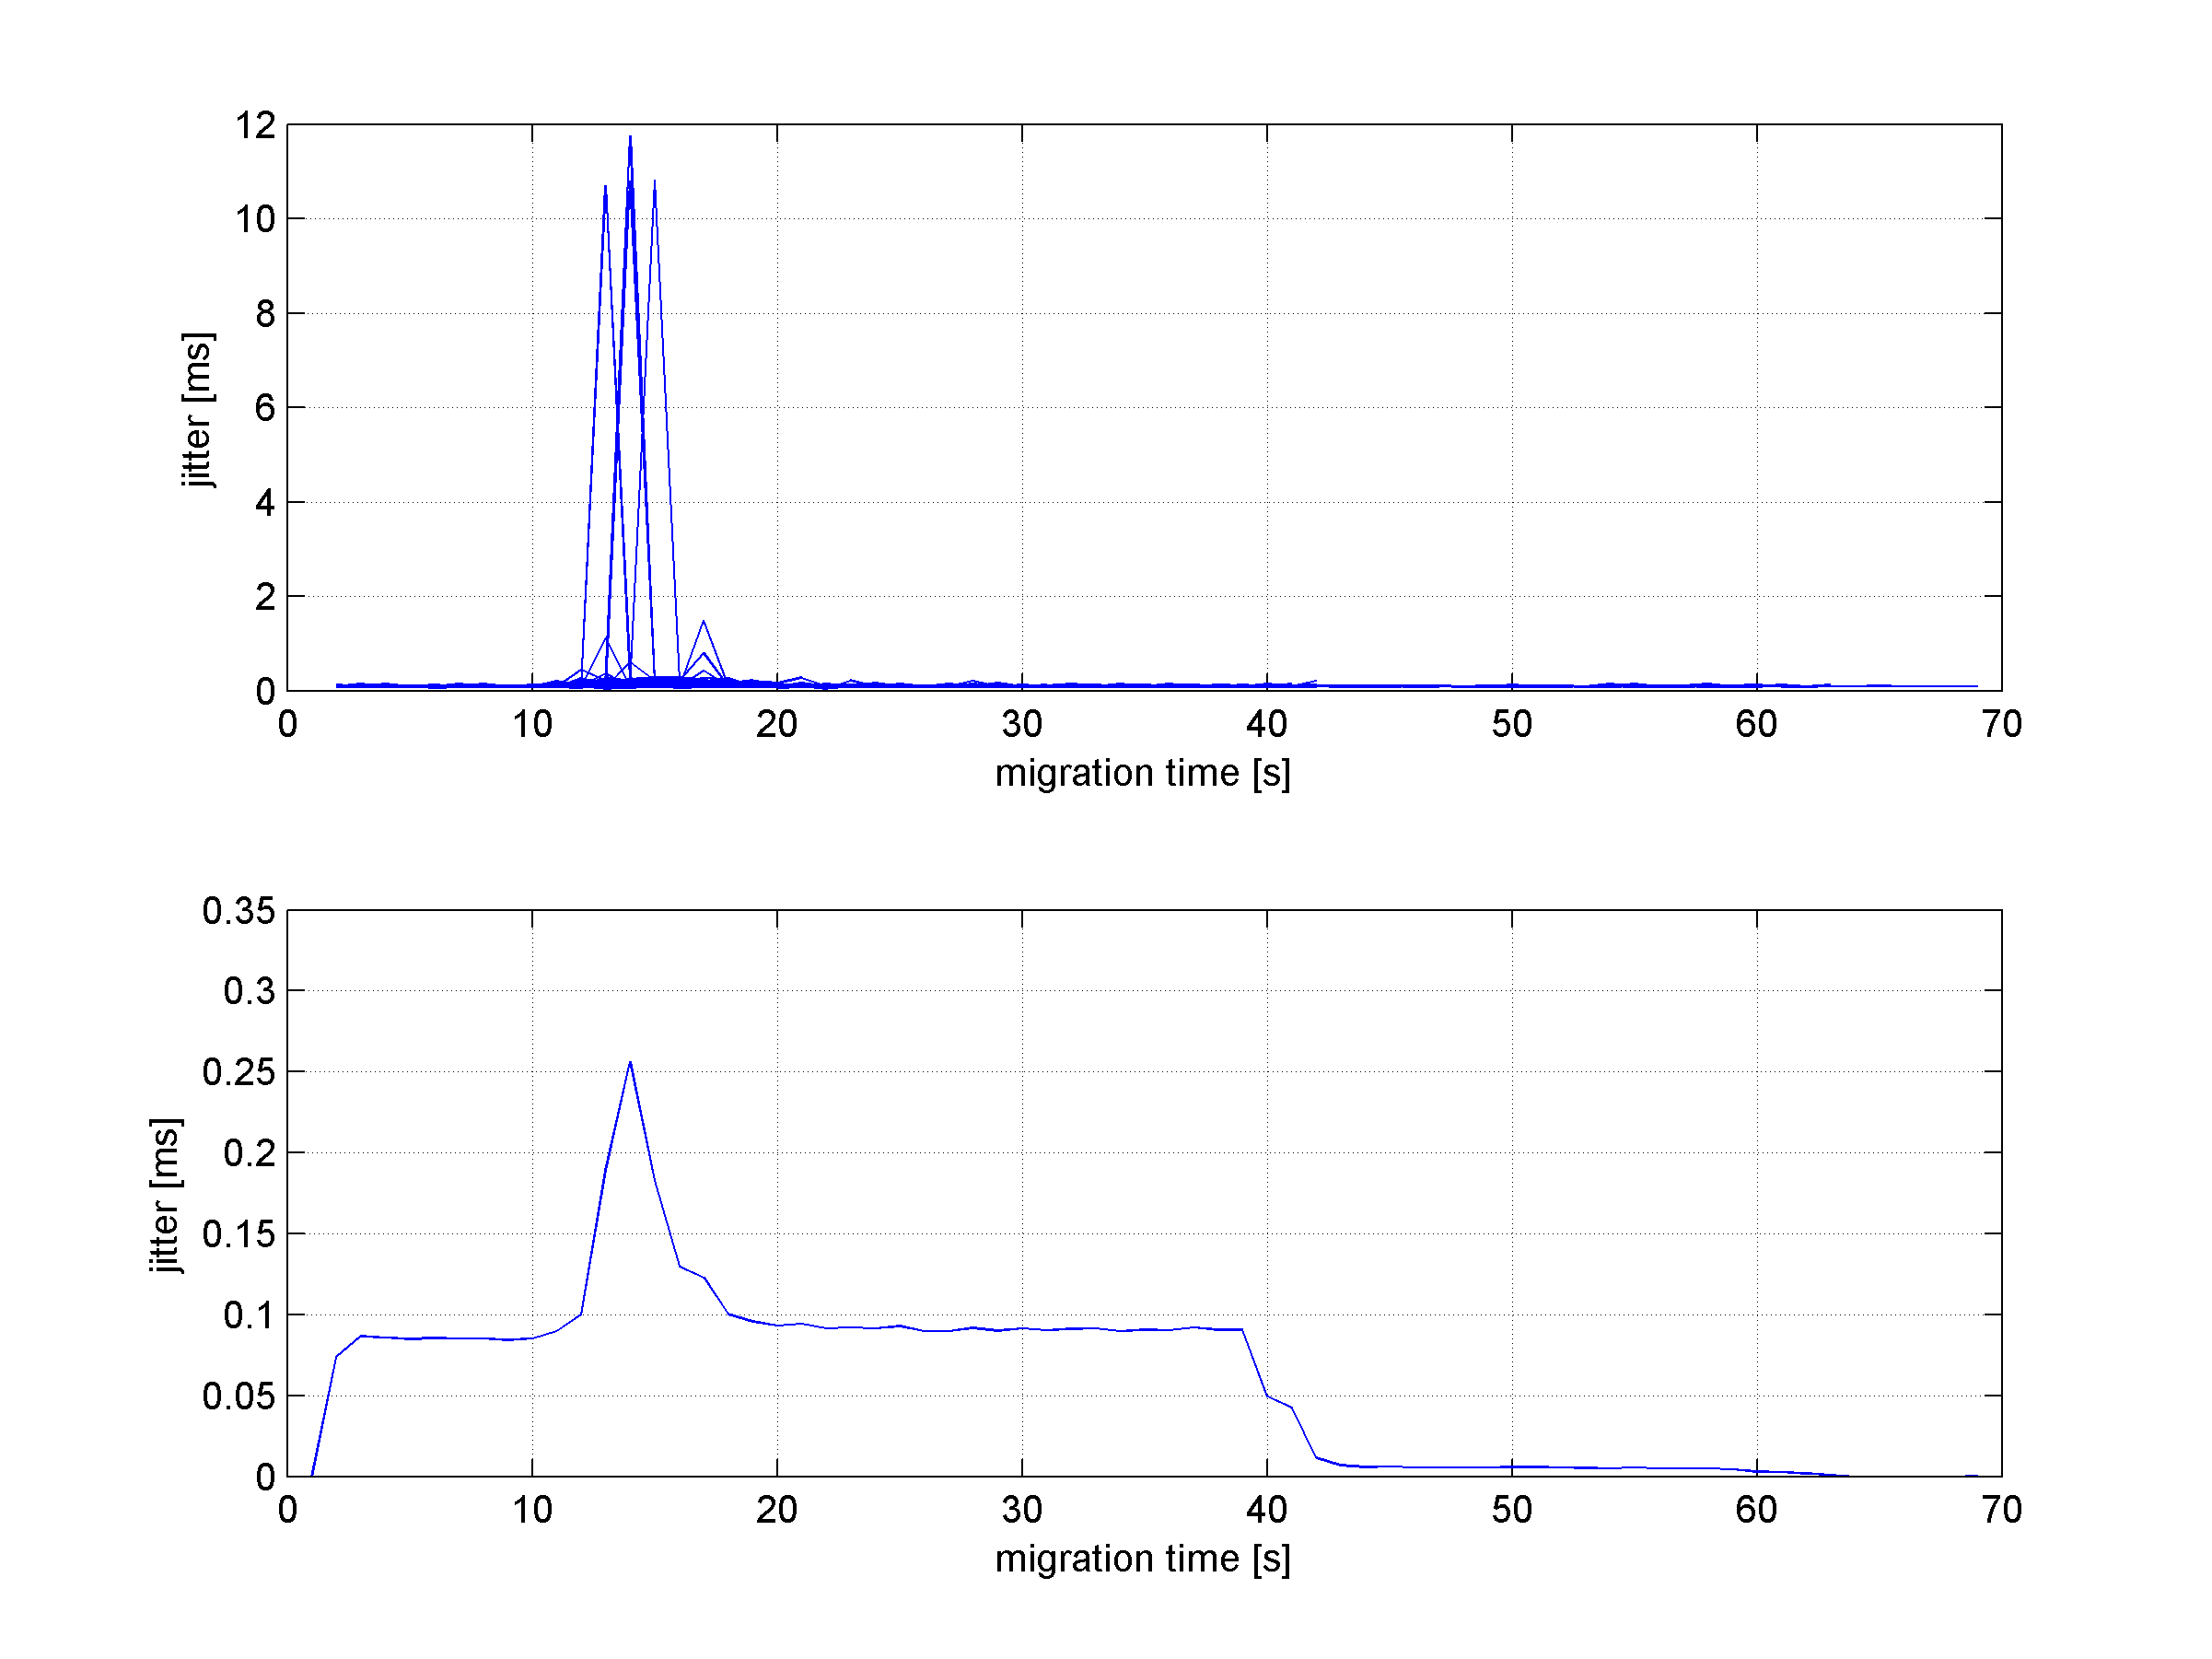
\includegraphics[width=0.9\textwidth]{results-274-all.png}
	\end{center}
	\caption[]{\#27, packet jitter for all sessions (top), average (bottom) [ms]}
	\label{img:results-274-all.png}
\end{figure}
\begin{figure}[hp]
	\begin{center}
	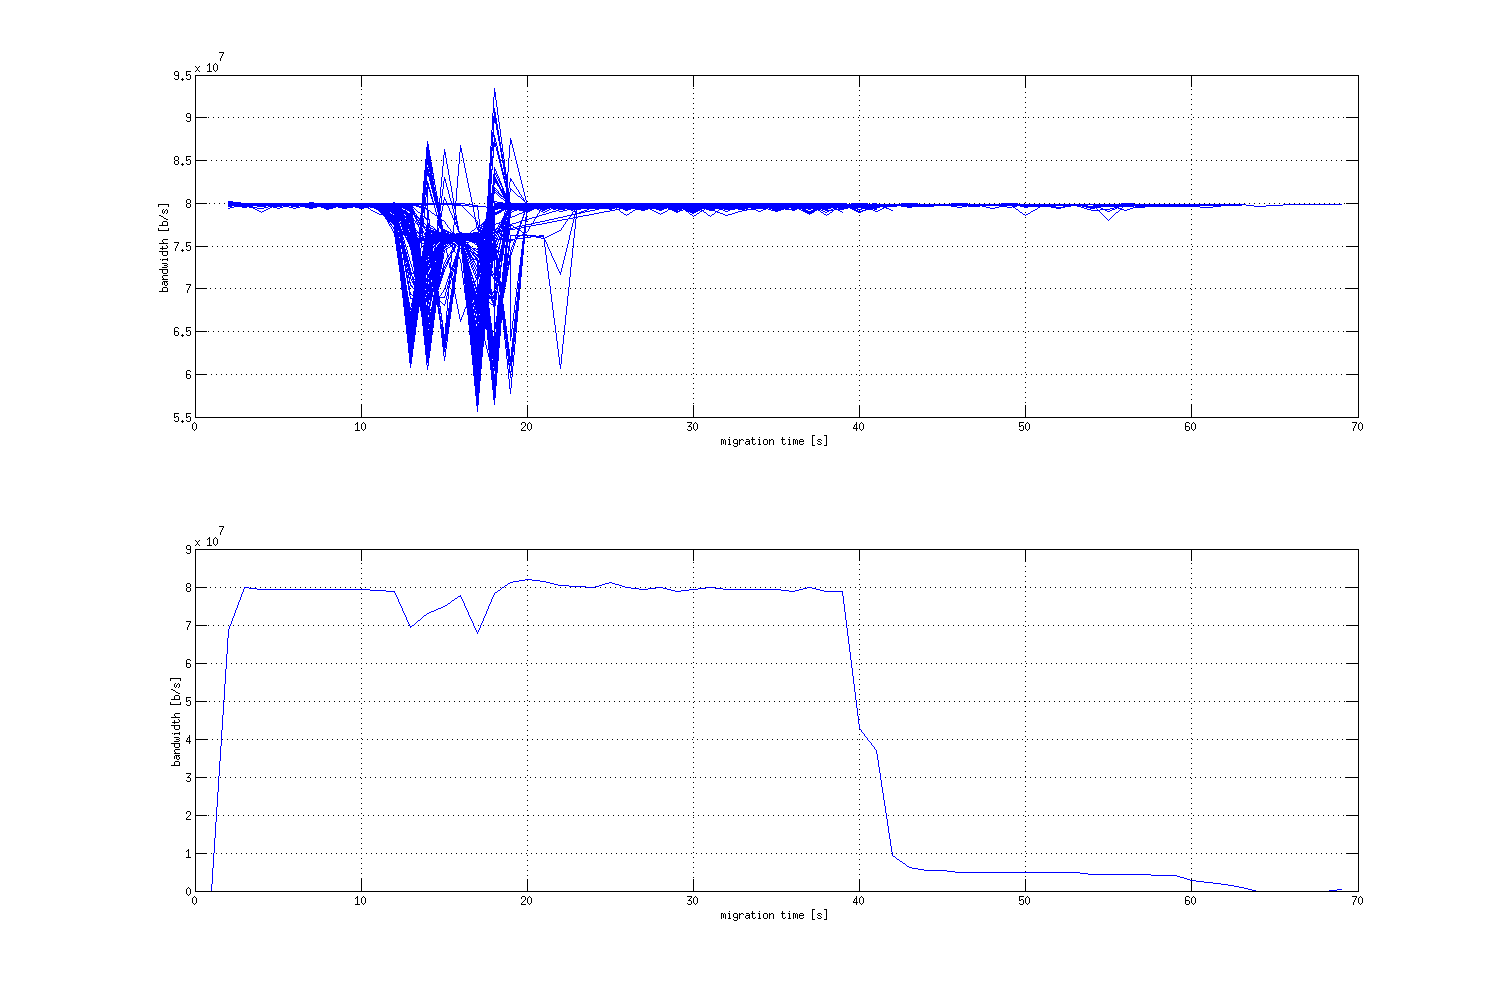
\includegraphics[width=0.9\textwidth]{results-279-all.png}
	\end{center}
	\caption[]{\#27, bandwidth for all sessions (top), average (bottom) [b/s]}
	\label{img:results-279-all.png}
\end{figure}
\begin{figure}[hp]
	\begin{center}
	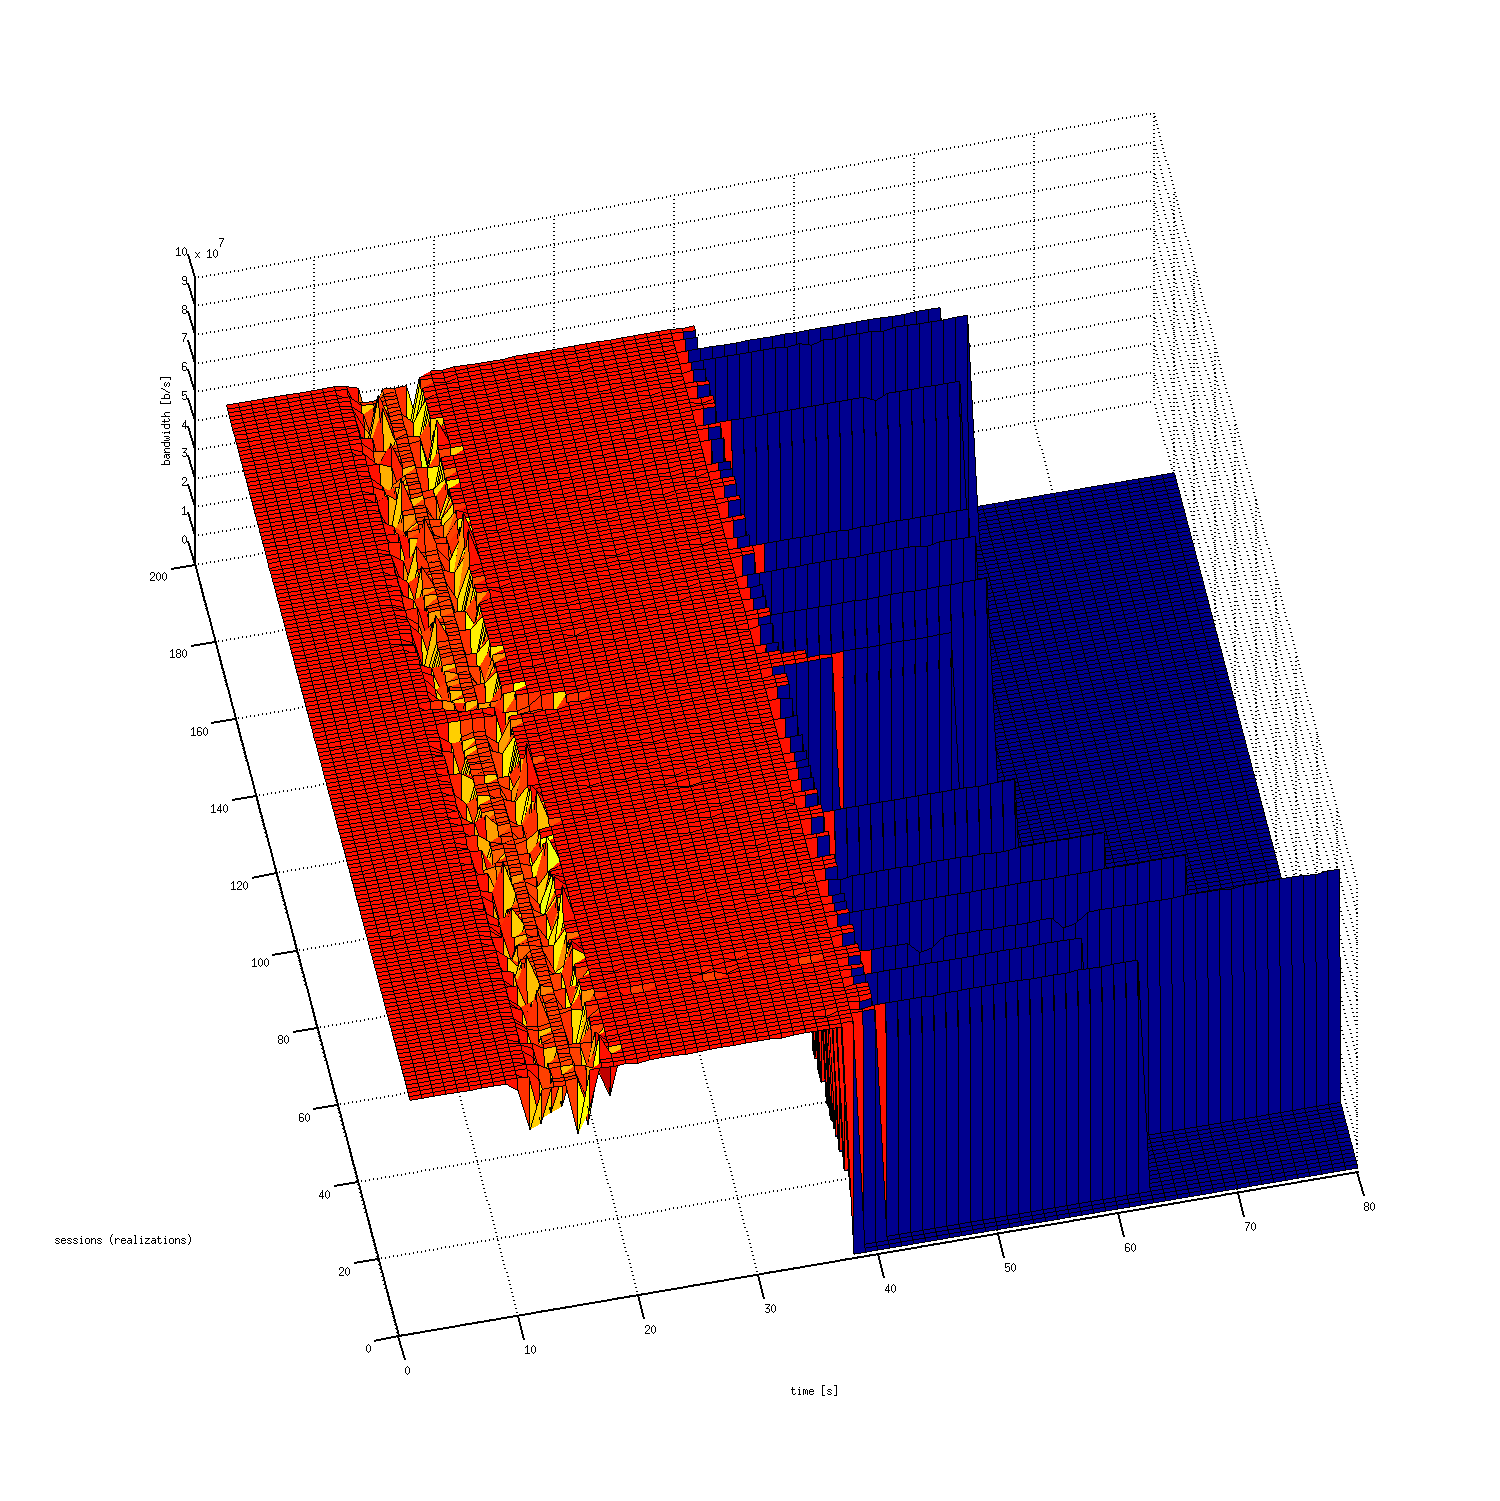
\includegraphics[width=0.9\textwidth]{results-279-3d.png}
	\end{center}
	\caption[]{\#27, bandwidth [b/s]}
	\label{img:results-279-3d.png}
\end{figure}
\begin{figure}[hp]
	\begin{center}
	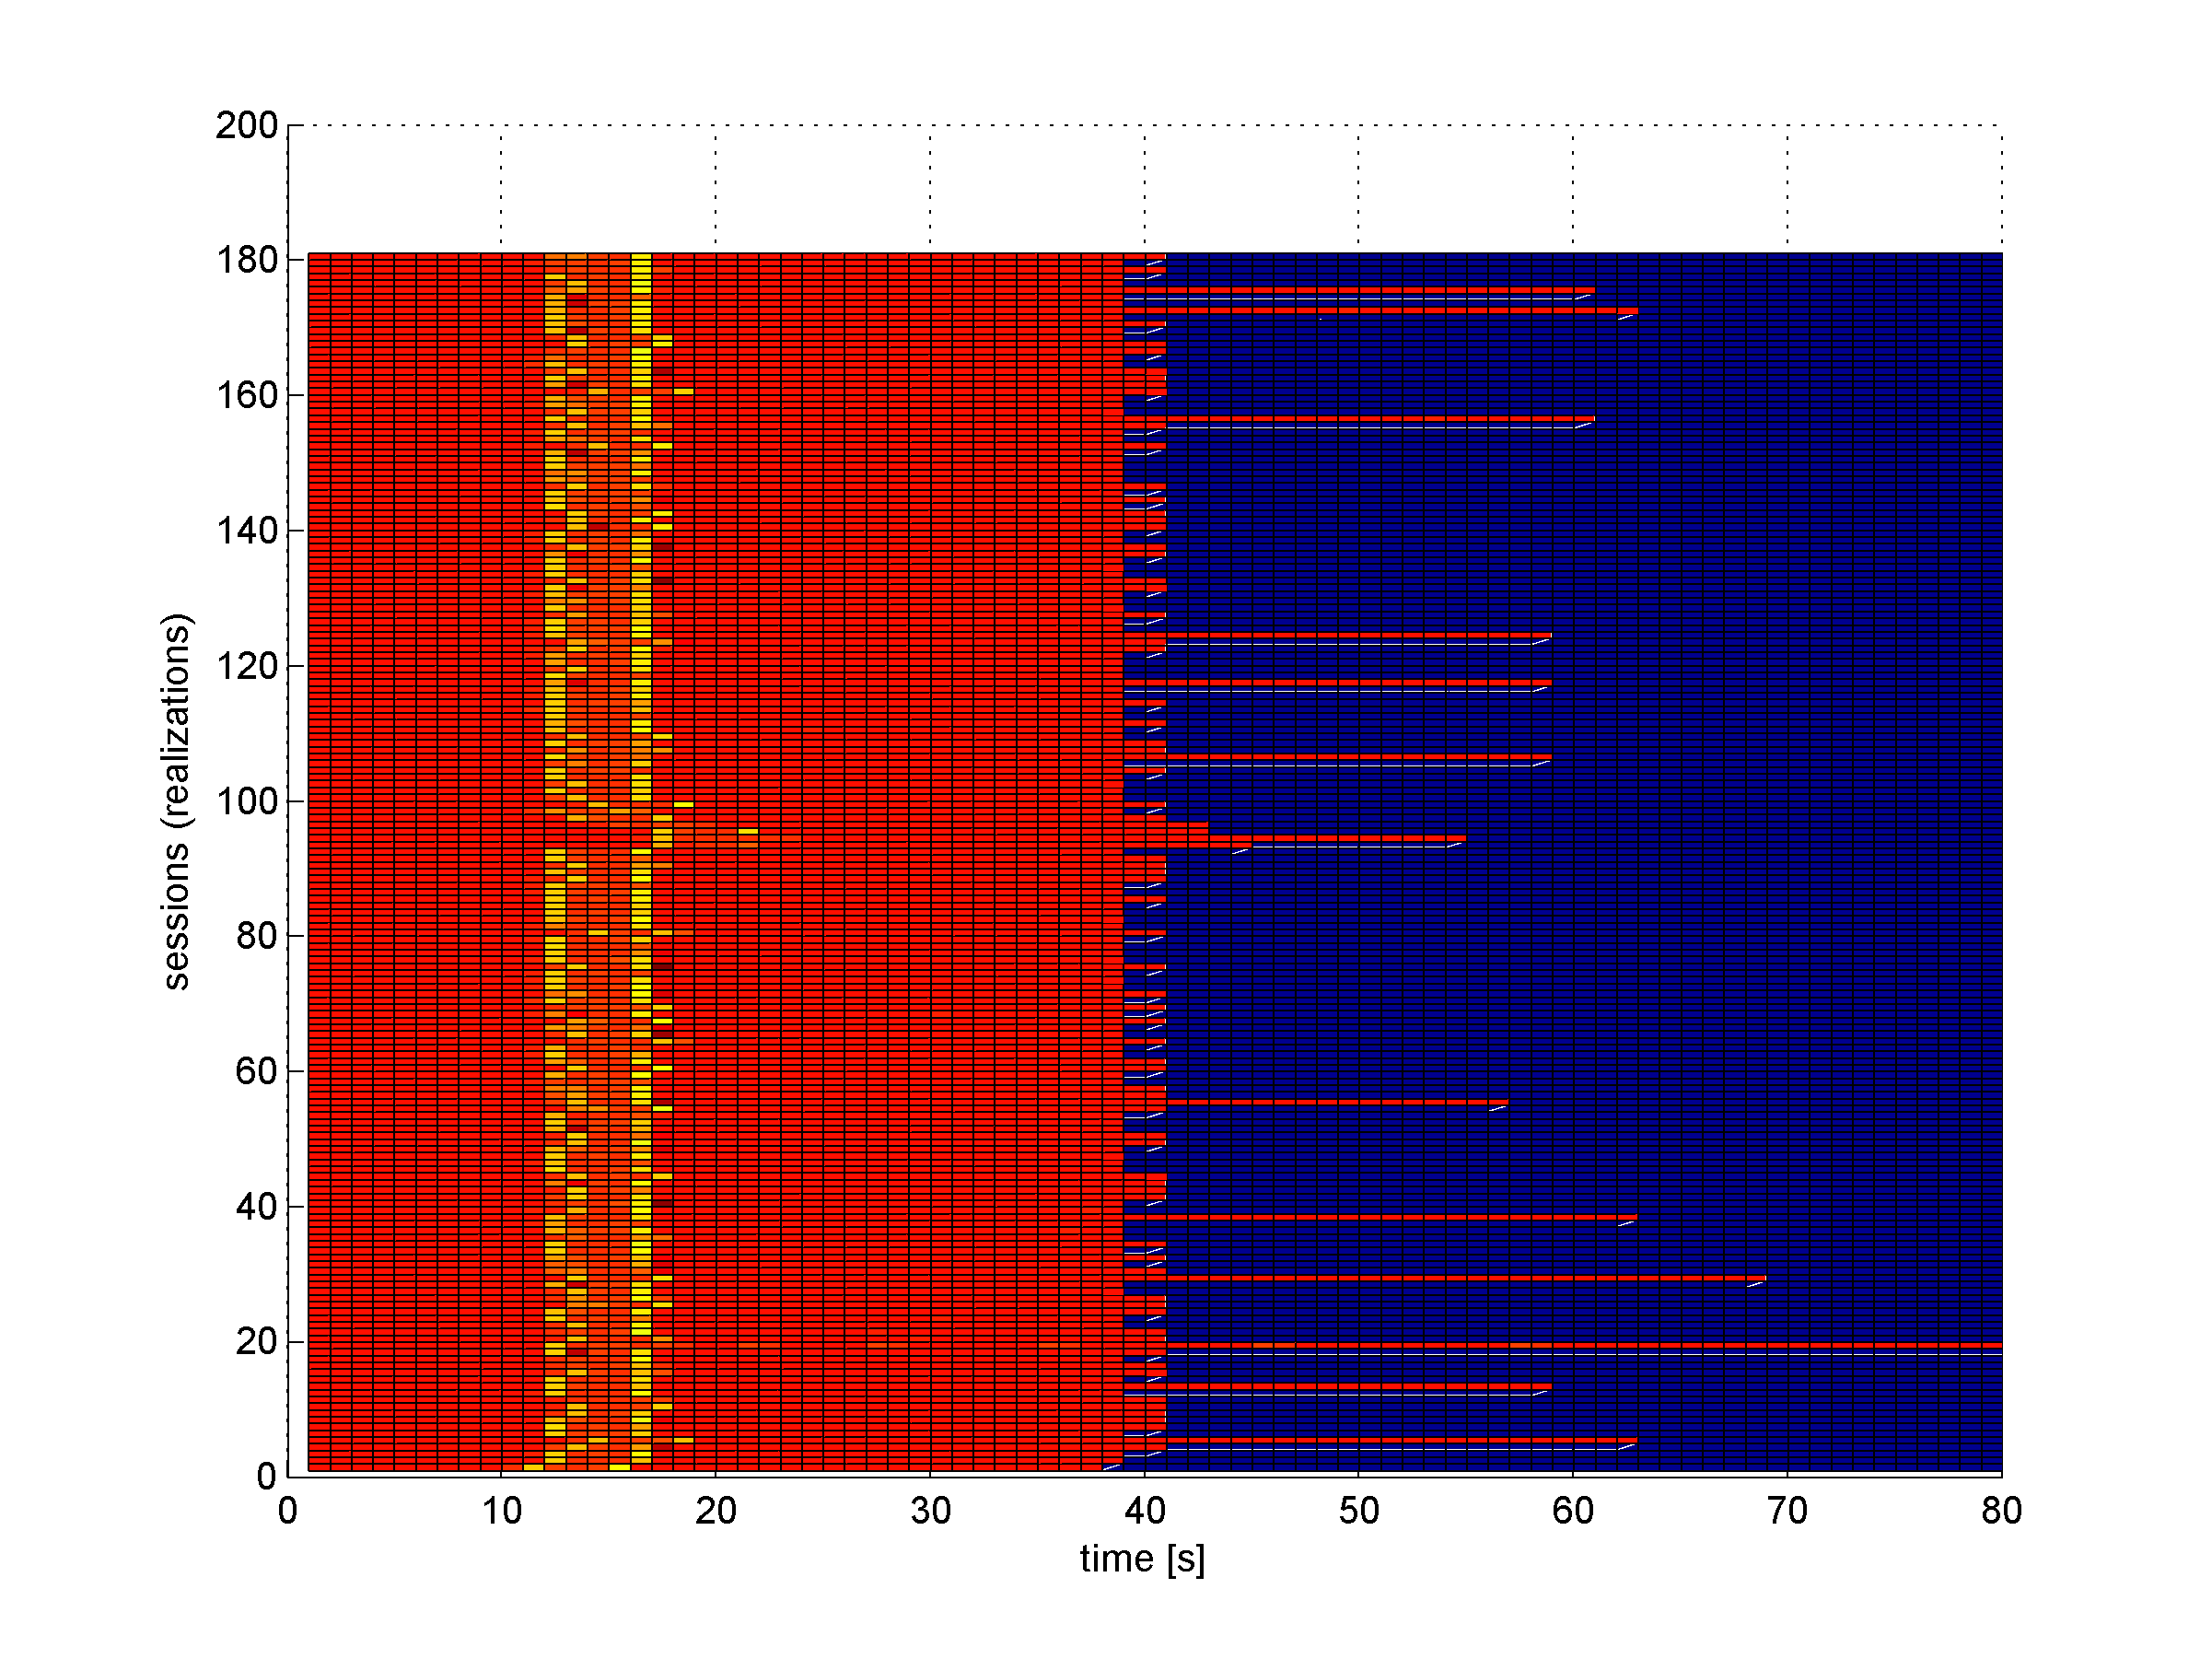
\includegraphics[width=0.9\textwidth]{results-279-2d.png}
	\end{center}
	\caption[]{\#27, bandwidth [b/s] (z axis - color), flat view}
	\label{img:results-279-2d.png}
\end{figure}
\FloatBarrier
